\documentclass{article}[12pt]
\renewcommand{\baselinestretch}{1.5}
\setlength{\parskip}{1em}

\usepackage[parfill]{parskip}
\usepackage[affil-it]{authblk}
\usepackage[space]{grffile}

\usepackage[a4paper]{geometry}
\usepackage[latin1]{inputenc}
\usepackage[english]{babel}

\geometry{verbose}
\usepackage{float}
\usepackage{graphicx}
\usepackage{setspace}
\usepackage{caption}

\usepackage{latexsym,textcomp,longtable,tabulary}
\usepackage{booktabs,array,multirow,braket}
\usepackage{amsfonts,amsmath,amssymb,mathbbol,calc,cancel}
\usepackage{subfigure,color,blindtext,enumitem,siunitx}
\usepackage[colorinlistoftodos]{todonotes}

\usepackage{mathtools}
\usepackage{url,hyperref,etoolbox}
\numberwithin{equation}{section}
\hypersetup{colorlinks=false,pdfborder={0 0 0}}

%+figure layout options
\restylefloat{figure}
\setlist{leftmargin=*,before=\setlength{\rightmargin}{\leftmargin}}
\graphicspath{{./figures/}{docs/figures/}}

\providecommand\citet{\cite}
\providecommand\citep{\cite}
\providecommand\citealt{\cite}

\makeatletter
\makeatother

\begin{document}
\newcommand{\rates}{F_{\theta}}
\newcommand{\tangent}{T_{\theta}}
\newcommand{\steadystates}{\partial S_{\theta}}

\newcommand{\Det}{\left| \frac{\partial\rates}{\partial u} \right|}
\newcommand{\measure}{\Psi_{\theta}}

\newcommand{\predictions}{\mathcal{P}}
\newcommand{\targets}{\mathcal{D}}
\newcommand{\loss}{L}

\newcommand{\Reals}{\mathbb{R}}

\title{Inference of Bifurcations with Differentiable Continuation}
\author{Gregory Szep$^{1,2}$, Neil Dalchau$^2$ and Attila Csikasz-Nagy$^{1,3}$}
\affil{$^1$King's College London, UK, $^2$Microsoft Research Cambridge, UK, $^3$Pazmany Peter Catholic University, Budapest, Hungary}
\date{\today} \maketitle

\begin{abstract}
    In this work we propose a gradient-based semi-supervised approach for matching target bifurcations with parameterised differential equation models. The cost function contains a supervised likelihood term that is maximal when predicted bifurcations match the targets, and an unsupervised correction term that encourages bifurcations by maximising the curvature of the determinant of the Jacobian. The calculation of gradients with respect to parameters shares the same computational complexity as deflated pseudo-arclength continuation used to calculate the bifurcation diagram. We demonstrate model synthesis with minimal models which explore the space of saddle-node and pitchfork diagrams, a genetic toggle switch from synthetic biology and the FitzHugh-Nagumo model. Furthermore, the cost landscape allow  us  to  organise  models  in  terms  of topological and geometric equivalence.
\end{abstract}

\section{Introduction}
\subsection{Background}

Backpropagation through differential equation solves has been a breakthrough over the past couple of years \cite{Chen2018NeuralEquations,Rackauckas2019DiffEqFlux.jl-AEquations} that enabled scalable parameter inference for differential equations. Optimisation targets, however, have mostly been expressed in the spatio-temporal domain. Acquisition of such data can be costly and can often contain over-constraining information generated by processing steps or the measurement device rather than the state variables that underpin the observed mechanism. In microscopy, for example, data is often reported in arbitrary fluoresce units allowing the observer to shift and scale data arbitrarily. Furthermore, such data may also not contain sufficient information about dynamical transients in order to identify kinetic parameters. The emerging picture suggests that identification of the qualitative dynamics -- the bifurcation diagram -- should precede any attempt at inferring kinetic parameters \cite{Stumpf2019ParameterBifurcations}. Techniques for back-propagating through implicit equation solvers have also been developed \cite{Look2020DifferentiableLayers,Bai2019DeepModels} although at the time of writing this paper, have not been applied to bifurcation diagrams.

In this work we propose a gradient-based semi-supervised approach that focuses on fitting qualitative dynamics, defined by state space structures, rather than kinetics. Drawing inspiration from implicit solvers \cite{Look2020DifferentiableLayers,Bai2019DeepModels} to calculate gradients we find that their computation shares the same  complexity as the algorithm used to calculate the bifurcation diagram. We use a predictor-corrector method called deflated pseudo-arclength continuation \cite{Farrell2016TheDiagrams,Veltz2019PseudoArcLengthContinuation.jl}, originally developed for partial differential equations. In the case of partial differential equations the computational complexity of calculating a single bifurcation diagram is not bounded since superpositions of localised solutions may give rise to uncountably many branches \cite{Avitabile2010ToEquation}. The complexity of computing a single branch, however, is bounded by the complexities of the chosen eigenvalue solver and corrector, and further decreased by adaptive stepping procedures \cite{Aruliah2016AlgorithmContinuation}.

We find that the cost function landscape contains basins that not only allow us to synthesise models with a desired bifurcation structure but also allow us to organise models in terms of topological and geometric equivalence. We discuss the relevance of this in model selection.

% \subsection{Related Works}
% \begin{itemize}
%     \item smooth and match estimator methods \cite{Ranciati2017BayesianParameters}
%     \item bifurcation inference using Mixed Integer Nonlinear Programming optimisation strategy \cite{Otero-Muras2018Optimization-basedModels}
% \end{itemize}

\clearpage
\section{Method}

\subsection{Problem Statement}
Suppose we parameterise a set of differential equations for states $u\in\Reals^N$ with a function $\rates$ in an unknown parameter space $\theta\in\Reals^M$. We would like these differential equations to obey a set of target bifurcations $\targets:=\{p_1\dots p_K\}$ along a known bifurcation parameter $p\in\Reals$. The following sections outline how a gradient descent algorithm could encourage predicted bifurcations $\predictions(\theta)$ coming from parameterised differential equations to match specified targets $\targets$. This would allow us to design differential equations using high-level qualitative constraints and sample qualitatively equivalent models in regions of optimal $\theta$. Let the differential equations be defined as
\begin{align}
	\partial_t u=\rates(z)
	\qquad\mathrm{where}\quad z:=(u,p)\quad
	\rates : \Reals^{N+1}\rightarrow\Reals^N
	\label{eq:model}
\end{align}

First we view the steady states of this problem in terms of implicit space curves \cite{Goldman2005CurvatureSurfaces} in an augmented state space $z\in\Reals^{N+1}$ which combines the state $u$ and bifurcation parameter $p$. We then realise that the curvature of the Jacobian determinant $\Det(z):=|\partial\rates/\partial u|$ is maximised when bifurcations appear in the observed region of $z$. Luckily the curvature can be evaluated analytically \cite{Goldman2005CurvatureSurfaces}. The steady state regions of $z$ are computed using a parameter continuation method \cite{Veltz2019PseudoArcLengthContinuation.jl,Farrell2016TheDiagrams}. Finally a differentiable semi-supervised cost function $\loss(\theta|\targets)$ is proposed that would allow gradient descent algorithms to efficiently encourage bifurcations and match their locations to targets $\targets$.

For clarity, we guide the reader through the methods with the following minimal models that explore the space of saddle-nodes $\rates(z) = p + \theta_{1}u+\theta_{2}u^3$ and pitchforks $\rates(z) = \theta_{1} + p u+\theta_{2}u^3$. These minimal models are shown with targets $\targets$ in Figure \ref{fig:saddle-node} and Figure \ref{fig:pitchfork} respectively. These figures show that the curvature of the determinant $\Det(z)$ increases in the vicinity of bifurcations and crosses zero at the bifurcations. This gives us our first hint of what should be optimised to encourage bifurcations. Success on these minimal models demonstrates the proof of concept, and success in practice is demonstrated on a genetic toggle switch model taken from synthetic biology and the FitzHugh-Nagumo model.
\begin{figure}[H]
\centering{}
\captionsetup{justification=centering}
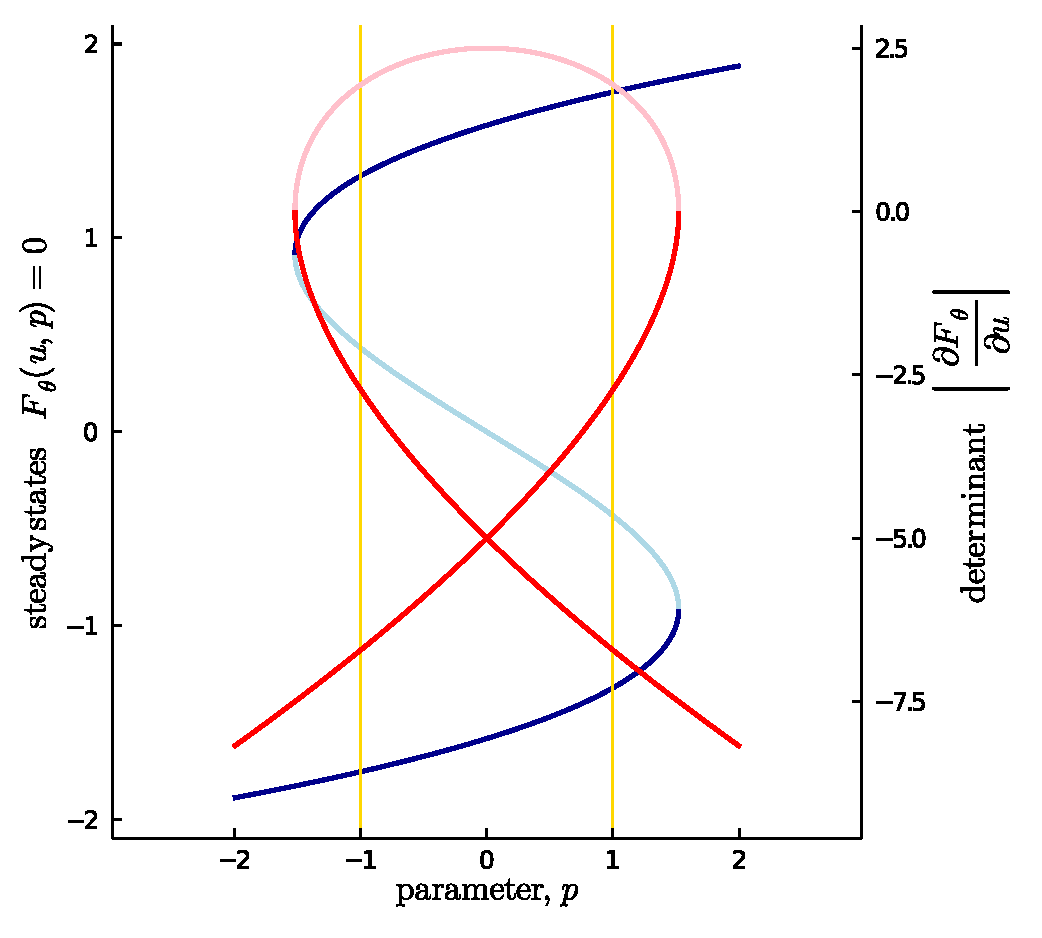
\includegraphics[width=11cm]{saddle-node}
\caption{Saddle-node model $\rates(z) = p + \theta_{1}u+\theta_{2}u^3$ with set $\theta=(2,-1)$ and targets $\targets=\{-1/2,1/2\}$. Lighter shades indicate the determinant crossing zero for unstable solutions}
\label{fig:saddle-node}
\end{figure}
\begin{figure}[H]
\centering{}
\captionsetup{justification=centering}
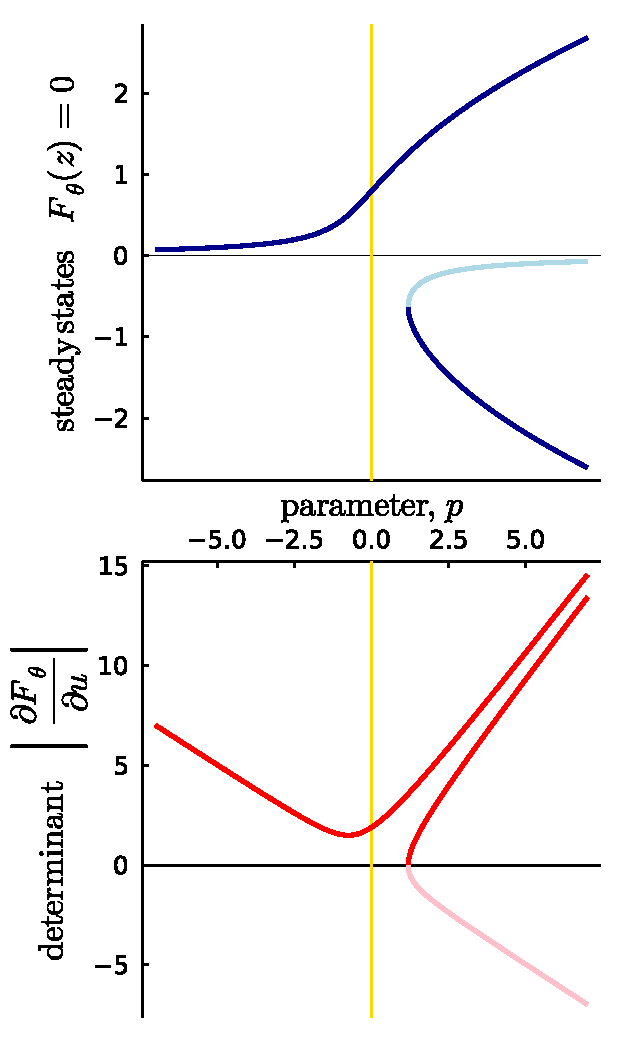
\includegraphics[width=11cm]{pitchfork}
\caption{Pitchfork model $\rates(z) = \theta_{1} + p u+\theta_{2}u^3$ with set $\theta=(-1/10,-1)$ and target $\targets=\{0\}$. Lighter shades indicate the determinant crossing zero for unstable solutions}
\label{fig:pitchfork}
\end{figure}

\subsection{Bifurcation Curves as Tangent Fields}
Suppose we want to find the intersection between $N$ surfaces where each surface is specified implicitly by a component of vector function $\rates:\Reals^{N+1}\rightarrow\Reals^N$. There are $N$ surfaces, each embedded in $\Reals^{N+1}$. Let's assume that their intersection exists and is not null or degenerate, then their intersection must be a set of one dimensional space curves in an augmented state space $z\in\Reals^{N+1}$ defined by
\begin{align}
    \rates(z) = 0
\end{align}
\begin{figure}[H]
\centering{}
\captionsetup{justification=centering}
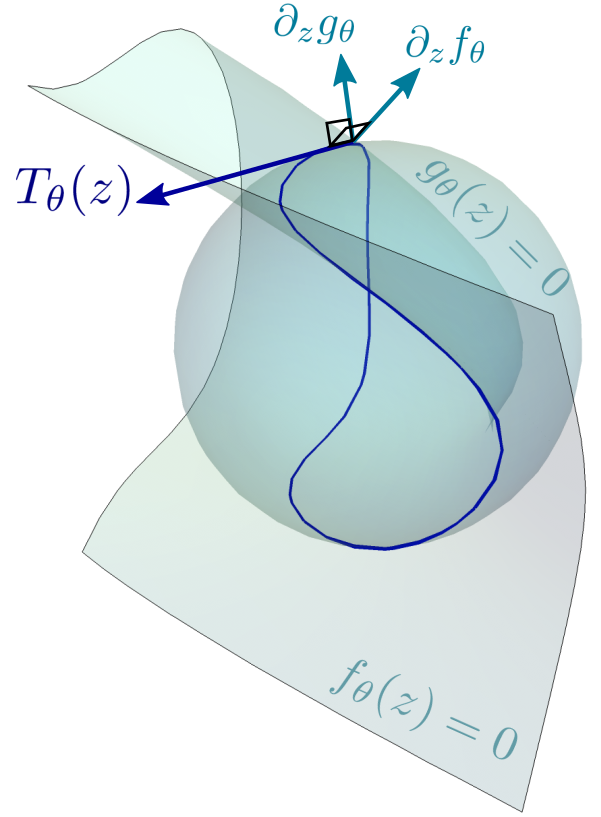
\includegraphics[width=5cm]{implicit-surfaces}
\caption{Two implicit surfaces $f_{\theta}(z)=0$ and $g_{\theta}(z)=0$ in $\mathbb{R}^3$ intersecting to form a\\ space curve which is tangent to field $\tangent(z)$ and perpendicular to gradients $\partial_{z}f_{\theta}$ and $\partial_{z}g_{\theta}$}
\label{fig:implicit-surfaces}
\end{figure}

An expression for the field $\tangent(z)$ tangent to the set of curves would allow us to take derivatives and integrals along them. Fortunately the tangent field can be constructed by ensuring it is perpendicular to the gradient $\partial_z$ of each component of $\rates$ as illustrated by an example two component system in Figure \ref{fig:implicit-surfaces}. The tangent field $\tangent(z)$ can be constructed perpendicular to all gradient vectors using the properties of the determinant \cite{Goldman2005CurvatureSurfaces}
\begin{align}
    \tangent(z):=
    \label{eq:tangent-field}
    \left|\begin{matrix}
        \hat{z} \\
        \,\partial_{z}\rates\,
    \end{matrix}\right|
    \qquad\tangent : \Reals^{N+1}\rightarrow\Reals^{N+1}\\
    =\sum_{i=1}^{N+1}\hat{z}_{i}(-1)^{i+1} \left|\frac{\partial \rates}{\partial(z\setminus z_{i}) }\right|
\end{align}
where $\hat{z}$ is a collection of unit basis vectors in the $\Reals^{N+1}$ space and $\partial_{z}\rates$ is an $N\times(N+1)$ rectangular Jacobian matrix of partial derivatives and $z\setminus z_{i}$ denotes the $N$ dimensional vector $z$ with component $z_{i}$ removed. This construction ensures that the dot product of this field any gradient of a component of $\rates$
\begin{align}
    \tangent(z)\cdot\partial_z f_{\theta} =
    \left|\begin{matrix}
        \partial_z f_{\theta} \\
        \,\partial_{z}\rates\,
    \end{matrix}\right|
    \quad =0 \quad\forall f_{\theta}\in \rates
\end{align}
since the determinant of any matrix with two identical rows or columns is zero. Note that the tangent field $\tangent(z)$ is actually defined for all values of $z$ where adjacent field lines trace out other level sets where $\rates(z)\neq0$. Furthermore deformations with respect to $\theta$ are always orthogonal to the tangent
% \todo{numerically true. analytic proof?}
\begin{align}
    \tangent(z)\cdot\frac{d\tangent}{d\theta}=0
\end{align}

\begin{figure}[H]
\centering{}
\captionsetup{justification=centering}
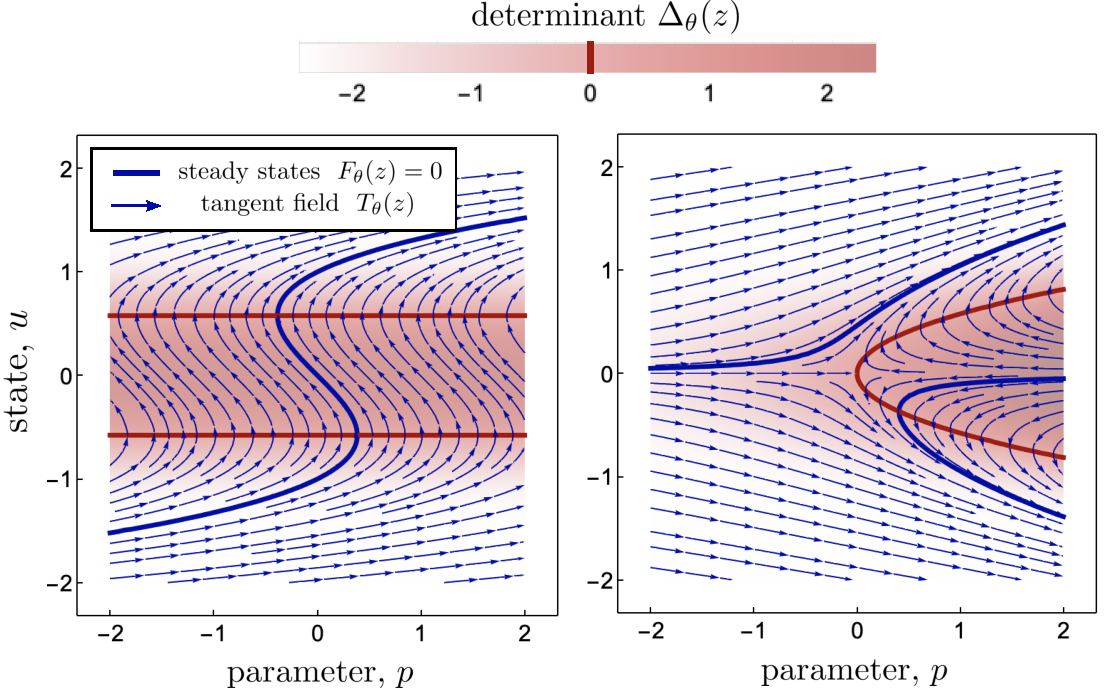
\includegraphics[width=14cm]{determinant-curvature}
\caption{Left/Right : Determinant $\Det(z)$ and tangent field $\tangent(z)$ for the saddle-node/pitchfork models for some set values of $\theta$ revealing that $\Det(z)=0$ defines bifurcations}
\label{fig:determinant-curvature}
\end{figure}

Figure \ref{fig:determinant-curvature} shows how the bifurcation curve defined by $\rates(z)=0$ picks out one of many traces in tangent field $\tangent(z)$ for the saddle and pitchfork. The tangent field $\tangent(z)$ can always be analytically evaluated by taking the determinant in \eqref{eq:tangent-field}. We will proceed with calculations on $\tangent(z)$ in the whole space $z$ and pick out a single trace by solving $\rates(z)=0$ later. For our two models
\begin{align}
    \underset{\mathrm{saddle-node\,\,model}}{
    \tangent(z)=\hat{u}-(\,3\theta_2 u^2+\theta_1\,)\,\hat{p}}
    \qquad\qquad
    \underset{\mathrm{pitchfork\,\,model}}{
    \tangent(z)=u\hat{u}-(\,3\theta_2 u^2+p\,)\,\hat{p}}
    \label{eq:tangent-field-examples}
\end{align}

\subsection{Evaluating Curvature of the Determinant}
Bifurcation points are defined as values of $z$ along the bifurcation curve where eigenvalues $\lambda$ of the Jacobian $\partial_u \rates(z)$ cross either the real or imaginary axis in the complex plane. Restricting our case to $\lambda\in\Reals$ for now, it would be sufficient to look for values of $z$ where one of the eigenvalues $\lambda$ crosses zero. Therefore the determinant of the Jacobian
\begin{align}
    \Det(z) := \left|\,\frac{\partial\rates}{\partial u}\,\right|
\end{align}
crossing zero can be used as a readout of whether a bifurcation has occurred. Figure \ref{fig:determinant-curvature} reveals this is indeed also true for any value $z$ --- not just along $\rates(z)=0$ --- for the saddle-node and pitchfork. The tangent field $\tangent(z)$ only folds when $\Det(z)=0$. Plotting the value of the determinant along $\rates(z)=0$ from Figure \ref{fig:determinant-curvature} would give rise to Figures \ref{fig:saddle-node} and \ref{fig:pitchfork}.

Consequently the curvature of the determinant $\partial_{\tangent}^2\Det$ along the tangent field $\tangent(z)$ in the vicinity of bifurcations tends to increase. Fortunately this curvature can always be obtained in closed analytical form. The second directional derivative with respect to tangent field $\tangent(z)$
\begin{align}
    \partial_{\tangent}^2\Det &:=
    \bigg(
        \partial_z\left(
            \partial_z\Det \cdot \hat{\tangent}
        \right)
    \bigg)\cdot \hat{\tangent}\quad
    \mathrm{where} \quad \hat{\tangent}:=\frac{\tangent}{|\tangent|}\\
    &=
    \hat{\tangent}\cdot\partial_z^2\Det\cdot\hat{\tangent}
    \quad+\quad
    \partial_z\Det\cdot\partial_z\hat{\tangent}\cdot\hat{\tangent}
    % & = \frac{1}{|\tangent|^2}\left(
    %     \tangent\cdot\partial_z^2\Det\cdot\tangent
    %     \quad+\quad
    %     \partial_z\Det\cdot
    %     \left(
    %     \mathbb{I}-\hat{\tangent}\hat{\tangent}^\top
    %     \right)\cdot\partial_z\tangent
    %     \cdot\tangent
    % \right)
\end{align}
The first term in the expression above is the usual result involving the Hessian matrix $\partial_z^2\Det$ when taking second order directional derivatives. The second term involving the gradient $\partial_z\Det$ appears because $\hat{\tangent}(z)$ is a function of $z$ giving rise to a non-zero Jacobian matrix $\partial_z \hat{\tangent}$. Using expressions for tangent fields \eqref{eq:tangent-field-examples} the determinant curvatures for our models become
\begin{align}
    \underset{\mathrm{saddle-node\,\,model}}{
    \partial_{\tangent}^2\Det =
    -\frac{6 \theta_2 \left(\theta _1^2-9 \theta _2^2 u^4+1\right)}
    {\left(\left(\theta _1+3 \theta _2 u^2\right){}^2+1\right){}^2}}
    \qquad
    \underset{\mathrm{pitchfork\,\,model}}{
    \partial_{\tangent}^2\Det =
    -\frac{2 u^2 \left(p+3 \theta _2 u^2\right) \left(9 \theta _2 \left(p+\theta _2 u^2\right)+1\right)}{
    ( \left(p+3 \theta _2 u^2\right)^2+u^2 )^2
    }}
\end{align}

\subsection{Semi-supervised Cost Function}

In order for predicted bifurcations $\predictions(\theta)$ to match targets $\targets$ we need to evaluate some form of error term on the bifurcation curve defined by $\rates(z)=0$. We can see from Figures \ref{fig:saddle-node} and \ref{fig:pitchfork} that predictions can be identified by look for points $p$ along the curve where the determinant $|\frac{\partial\rates}{\partial u}|=0$. We can constrain the cost function to be evaluated in the vicinity of predicted bifurcation points by weighting the likelihood by a function $\omega_\theta(z|\alpha)$ sharply peaked where $|\frac{\partial\rates}{\partial u}|=0$ and going to zero elsewhere. Similarly, we can construct a mixture distribution $\mathcal{N}(p|\targets,\varepsilon)$ peaking at the locations of targets $\targets$ and falling to zero elsewhere. If we choose Gaussian basis functions for both the target mixture and prediction weighting, the likelihood $L_{\theta}(z|\targets)$ takes the form
\begin{align}
    L_{\theta}(z|\targets) := 
    \lim_{\alpha\rightarrow\infty}\frac{\omega_\theta(z|\alpha)\,\mathcal{N}(p|\targets,\varepsilon)}{\int_{\rates(z)=0} \omega_\theta(z|\alpha)\,\mathrm{d}z}\label{eq:likelihood}\qquad\qquad\qquad\\
    \mathcal{N}(p|\targets,\varepsilon):=\frac{\sum_{p'\in\targets}\mathbb{e}^{-|p'-p|^2/\varepsilon}}{|\targets|\sqrt{\varepsilon\pi}}
    \quad
    \omega_\theta(z|\alpha):= \mathbb{e}^{-\alpha\left|\frac{\partial F_{\theta}}{\partial u}\right|^2}
\end{align}
where $\varepsilon$ and $\alpha$ are precision hyper-parameters. Figure \ref{fig:likelihood} shows how the likelihood $L_{\theta}(z|\targets)$ along the curve is indeed maximal when the bifurcations $\predictions(\theta)$ of the saddle-node model match the targets $\targets$.

Alpha justified as being large by balance between numerical instability due to normalisation and desire to constrain the loss to regions where determinant is zero.

\begin{figure}[H]
\centering{}
\captionsetup{justification=centering}
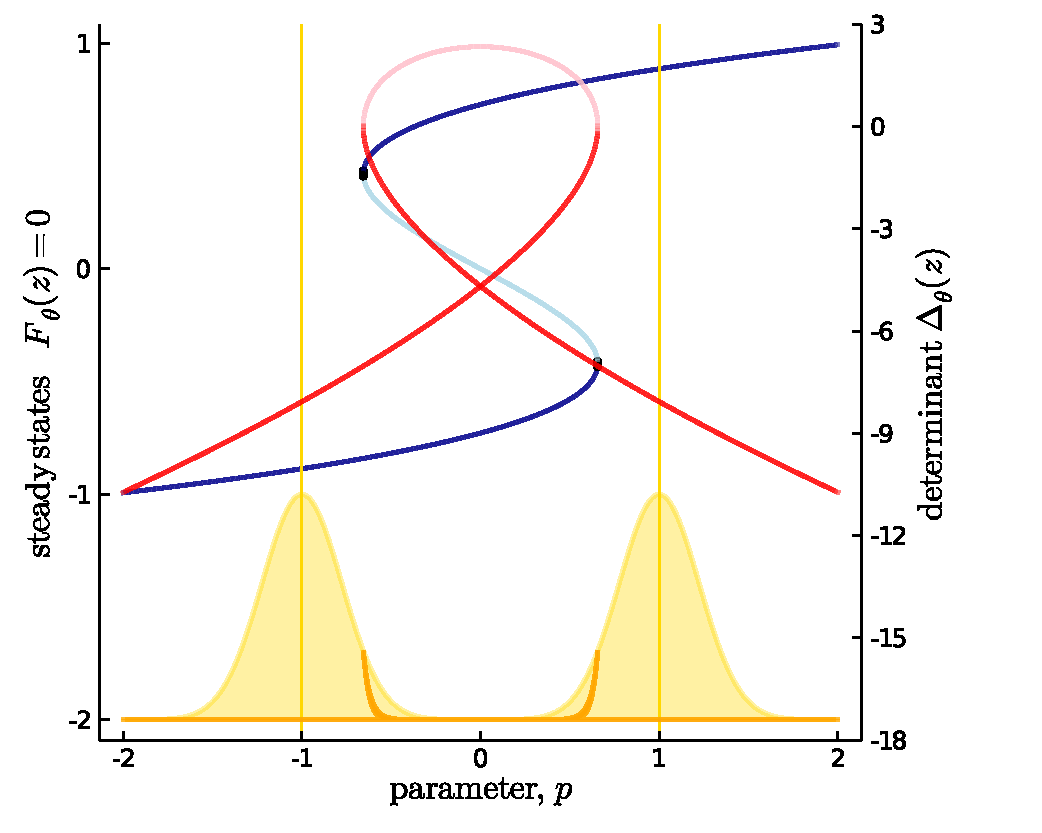
\includegraphics[width=7cm]{likelihood-1.pdf}
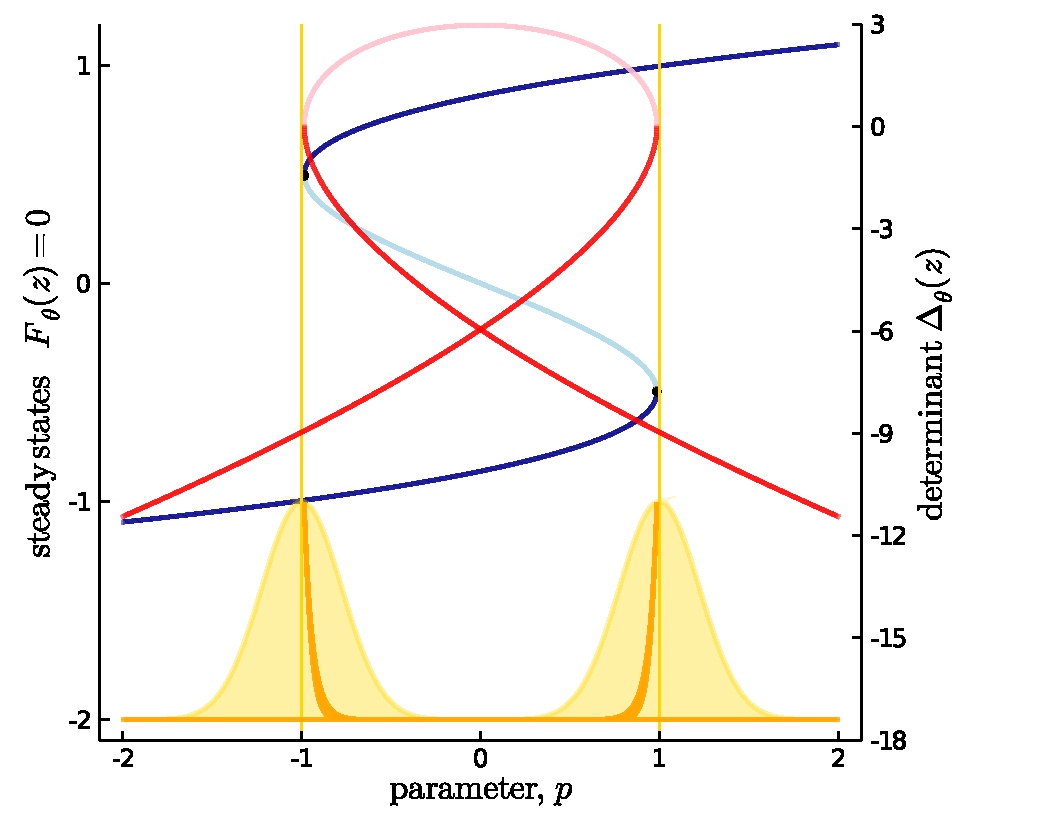
\includegraphics[width=7cm]{likelihood-2.pdf}
\caption{Likelihood $L_{\theta}(z|\targets)$ shown in dark gold is sharply peaked around the bifurcation points $\predictions(\theta)$ and is maximal when they match the targets (Right). The light gold envelope shows the maxima of the likelihood as the points $\predictions(\theta)$ sweep across different values of $p$}
\label{fig:likelihood}
\end{figure}

But what should the likelihood term \eqref{eq:likelihood} look like if there are no or fewer bifurcations than targets present in the observed region of $p\in\Omega$? This is where the curvature of the determinant $\partial_{\tangent}^2\Det$ can be extremised to encourage bifurcations. We can treat this curvature as an unsupervised correction of magnitude $\lambda$ to a supervised likelihood $L_{\theta}(z|\targets)$. We are now ready to write down the semi-supervised cost function for a bifurcation curve defined by $\rates(z)=0$ in an observed region $p\in\Omega$ as the negative log-likelihood
\begin{align}
    \loss(\theta|\targets,\Omega) := -\log\left(\int_{\partial S}
    L_{\theta}(z|\targets) + \lambda\,K_{\theta}(z)^2\,
    \,\mathrm{d}z\right)\qquad
     K_{\theta}(z):=\frac{\partial^2\Det}{\partial\tangent^2}\\
     \partial S := \{ (u,p) : \rates(u,p)=0, p\in\Omega \}
     \qquad\qquad\qquad\qquad
\end{align}
Both $L_{\theta}(z|\targets)$ and $K_{\theta}(z)$ have explicit analytic expressions and therefore can be differentiated easily. The integration region $\partial S$ is specified implicitly and in most cases will require a numerical procedure to find the roots $\rates(z)=0$ in the region $p\in\Omega$. In a similar vein to back-propagation through neural differential equations \cite{Chen2018NeuralEquations} we would like to be able to differentiate the cost $\loss(\theta|\targets,\Omega)$ without having to differentiate through the operations of the solver that finds $\rates(z)=0$. Fortunately this is all possible if we apply a similar strategy to that used by implicit layers \cite{Look2020DifferentiableLayers}; see Appendix \ref{appendix:space-curve} and \ref{appendix:deformation} for derivations.

% \subsection{Basis Functions and Unsupervided Bias}
% \subsection{Pseudo-arclength Continuation}

\subsection{Implementation}
Here provide a high-level view of Algorithm \ref{alg:optimisation-loop}. We use \texttt{BifurcationKit.jl} \cite{Veltz2019PseudoArcLengthContinuation.jl} to calculate bifurcation diagrams, which requires the rate function $\rates$, its Jacobian $J_\theta$ which can be calculated using \texttt{ForwardDiff.jl} \cite{Revels2016Forward-ModeJulia}, and an initial guess $u_0$ at an initial parameter $p_0$. Let this algorithm be called by function \texttt{getSteadyStates} and return the steady states that form the integration region $\partial S$ and a new guess $u_0$ that is the true steady state at $p_0$.

The algorithm also takes hyperparameters $\beta$ which will contain arclength step sizes, eigenvalue and Newton solver options and unsupervised correction factor $\lambda$. The adaptive hyperparameter update is done by \texttt{updateHyperparameters} and should depend on the current solutions $\partial S$ and the targets $\targets$. The step sizes and solver options should adapt to the expected space of the solutions $\partial S$ so that the waiting time between iterations is minimised. The unsupervised correction factor $\lambda$ should be large when there are no predicted bifurcations and decrease as the number of predicted bifurcations approaches the number of targets.

The evaluation of the cost gradient is done by \texttt{costGradient} using \texttt{ForwardDiff.jl} \cite{Revels2016Forward-ModeJulia} which has a large repository of chain rules that it uses to correctly evaluate derivatives. At the time of writing this paper the repository does not include the Leibniz rule \cite{Flanders1973DifferentiationSign} for implicitly defined line integrals, and we therefore define additional rules that implement the results shown in Appendix \ref{appendix:space-curve} and \ref{appendix:deformation}. The cost gradient is used by \texttt{updateParameters}, which can be any gradient-based optimiser such as ADAM or Momentum gradient decent, to update the parameters $\theta$.
\\\\
\begin{algorithm*}[H]
\label{alg:optimisation-loop}
\SetAlgoLined
\textbf{Inputs} Function $F_{\theta}:\mathbb{R}^{N+1}\rightarrow\mathbb{R}^{N}$ for $u\in\mathbb{R}^N$ and $p\in\mathbb{R}$\\ target bifurcations $\mathcal{D}=\{p_1\dots p_K:p\in\Omega\}$ and convergence tolerance $\varepsilon$\\
\textbf{Output} Optimised $\theta\in\mathbb{R}^M$ that satisfy targets $\targets$\\
$u_0\leftarrow\mathrm{rand}\in\mathbb{R}^{N}$\quad\,$\theta\leftarrow\mathrm{rand}\in\mathbb{R}^{M}$\\
$\beta\leftarrow\texttt{getHyperparameters}(\targets)$\\
\While{$\mathrm{tolerance}(\beta)>\varepsilon$}{
  $\partial S,u_0\leftarrow\texttt{getSteadyStates}(F_{\theta},u_0,\beta)$\\
  $\beta\leftarrow\texttt{updateHyperparameters}(\beta,\partial S,\targets)$\\
  $\partial L\leftarrow\texttt{costGradient}(F_{\theta},\partial S,\targets,\beta)$\\
  $\theta\leftarrow\texttt{updateParameters}(\theta,\partial L,\beta)$
}
\caption{Bifurcation Optimisation Loop}
\end{algorithm*}

\section{Results}

\subsection{Minimal Models}
Figures \ref{fig:saddle-node:results} and \ref{fig:pitchfork:results} show example optimisations of $(\theta_1,\theta_2)$ for the minimal saddle-node and pitchfork models respectively. The magnitude of the correction factor $\lambda=0$ when bifurcations are present and $\lambda\neq0$ otherwise.

\begin{figure}[H]
\centering{}
\captionsetup{justification=centering}
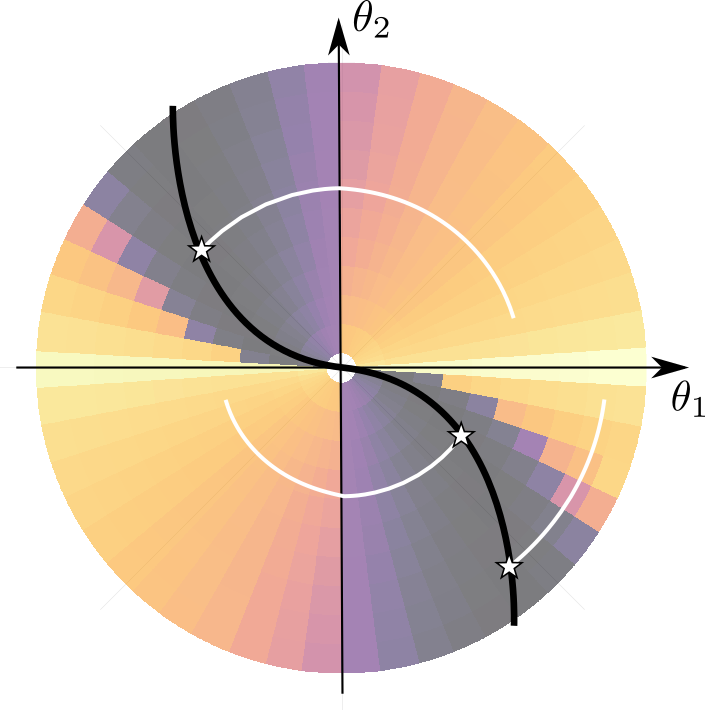
\includegraphics[width=6cm]{saddle-landscape.png}
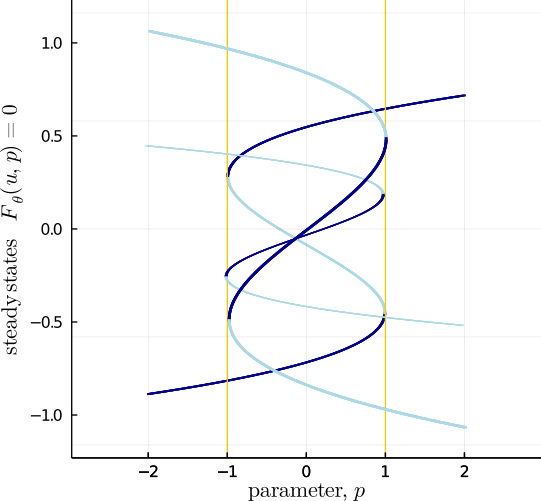
\includegraphics[width=6cm]{saddle-optima.png}
\caption{Saddle-node model $\rates(z) = p + \theta_{1}u+\theta_{2}u^3$ optimised with respect to targets $\targets=\{-1,1\}$ in observation region $\Omega\in[-2,2]$. Left panel: trajectories in white approaching black line of global optima.}
\label{fig:saddle-node:results}
\end{figure}

\subsection{Hyperparameters}
Discuss $\alpha$, $\varepsilon$ and $\lambda$.

\subsection{Applied Models}
In progress...
\begin{itemize}
    \item Genetic toggle switch
    \item FitzHugh-Nagumo
\end{itemize}
% \subsubsection{Genetic toggle switch}
% \subsubsection{FitzHugh-Nagumo}


% \begin{equation}
%     \dfrac{du_1}{dt} = \dfrac{a_1} { 1 + (p u_2)^2 } - \mu_1 u_1, \quad
%     \dfrac{du_2}{dt} = \dfrac{a_2} { 1 + (k u_1)^2 } - \mu_2 u_2
% \end{equation}
% Without loss of generality, we can rescale $u_1$ by $a_1$ and $u_2$ by $a_2$:
% \begin{equation*}
%     \dfrac{du_1}{dt} = \dfrac{1} { 1 + (\hat{p} u_2)^2 } - \mu_1 u_1, \quad
%     \dfrac{du_2}{dt} = \dfrac{1} { 1 + (\hat{k} u_1)^2 } - \mu_2 u_2
% \end{equation*}
% where $\hat{p} = p a_2$ and $\hat{k} = k a_1$. The equilibria for this system are defined by
% \begin{equation}
%     \mu_1u_1^*(1+\hat{p}u_2^*)^2 = 1, \quad \mu_2u_2^*(1+\hat{k}u_1^*)^2 = 1
% \end{equation}
% Obtaining closed form expressions for $u_1^*$ and $u_2^*$ requires solving a quintic polynomial. We won't do that here.

% What is the determinant for this system?
% \begin{equation*}
%     \left|\dfrac{\partial F}{\partial u}\right| = 
%     \begin{vmatrix} -\mu_1 & -\frac{2 p^2 u_2^*}{(1 + (p u_2^*)^2)^2} \\
%         -\frac{2k^2u_1^*}{(1+(k u_1^*)^2)^2} & -\mu_2
%     \end{vmatrix}
%     = \mu_1\mu_2 - \frac{4p^2k^2u_1^*u_2^*}{(1+(p u_2^*)^2)^2(1+(k u_1^*)^2)^2}
% \end{equation*}

% \subsubsection{Two-state (generalised)}
% \begin{equation}
%     \dfrac{du_1}{dt} = \dfrac{a_1 + b_1(p u_2)^2} { 1 + (p u_2)^2 } - \mu_1 u_1, \quad
%     \dfrac{du_2}{dt} = \dfrac{a_2 + b_2(k u_1)^2} { 1 + (k u_1)^2 } - \mu_2 u_2
% \end{equation}

% Applying the same rescaling as above, we can simplify as
% \begin{equation}
%     \dfrac{du_1}{dt} = \dfrac{1 + \rho_1(p u_2)^2} { 1 + (p u_2)^2 } - \mu_1 u_1, \quad
%     \dfrac{du_2}{dt} = \dfrac{1 + \rho_2(k u_1)^2} { 1 + (k u_1)^2 } - \mu_2 u_2
% \end{equation}
% where $\rho_i = \frac{b_i}{a_i}$, with other parameters rescaled as above (but dropping hats).


\subsection{Computational Complexity}

% \section{Discussion}
% \label{sec:discussion}

% \subsection{Model Synthesis}
% \subsection{Model Selection}

\appendix
\appendixpage
\addappheadtotoc
\section{Supplementary Figures}

\begin{figure}[H]
\centering
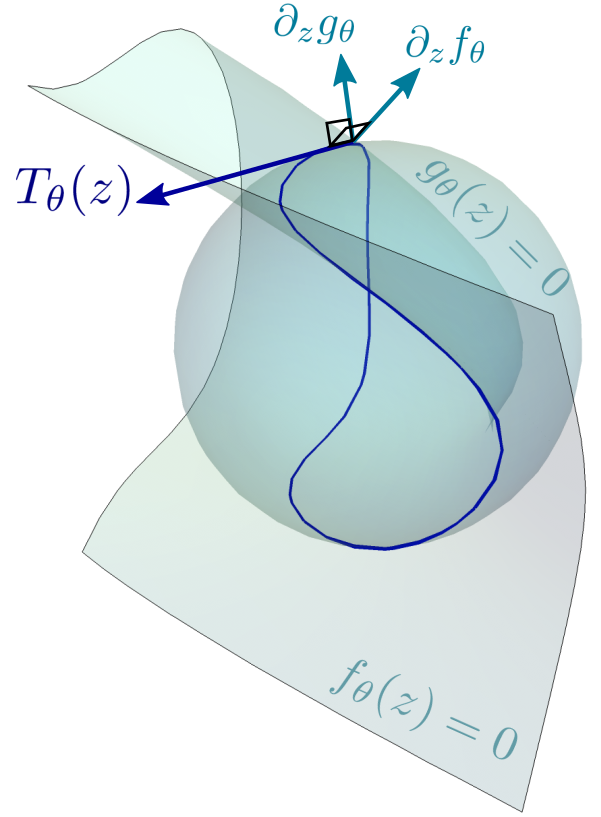
\includegraphics[width=5cm]{implicit-surfaces}
\caption{Two implicit surfaces $f_{\theta}(z)=0$ and $g_{\theta}(z)=0$ in $\mathbb{R}^3$ intersecting to form a space curve which is tangent to field $\tangent(z)$ and perpendicular to gradients $\partial_{z}f_{\theta}$ and $\partial_{z}g_{\theta}$}
\label{fig:implicit-surfaces}
\end{figure}

\section{Gradient of Space Curve}
\label{appendix:space-curve}

Suppose there exists a one dimensional space curve $\mathcal{C(\theta)}$ embedded in $z\in\Reals^{N+1}$ whos geometry changes depending on input parameters $\theta\in\Reals^M$. This curve could be open or closed and changes in $\theta$ could change the curve topology as well. Let the function $\gamma_{\theta}:\Reals\rightarrow\Reals^{N+1}$ be a parameterisation of the position vector along the curve within a fixed domain $s\in\mathcal{S}$. Note that the choice of parameterisation is arbitrary and our results should not depend on this choice. Furthermore, if we parametrise the curve $\mathcal{C}(\theta)$ with respect to a fixed domain $\mathcal{S}$ the dependence on $\theta$ is picked up by the parameterisation $\gamma_{\theta}(s)$. We can write a line integral of any scalar function $L_{\theta}:\Reals^{N+1}\rightarrow\Reals$ on the curve as
\begin{align}
    L(\theta):=
    \int_\mathcal{C(\theta)}\! L_{\theta}(z)\,\mathrm{d}z
    =\int_\mathcal{S}\! L_{\theta}(z)\left|\frac{d\gamma_{\theta}}{ds}\right|\mathrm{d}s_{\,\,z=\gamma_{\theta}(s)}
\end{align}
where $\left|\frac{d\gamma_{\theta}}{ds}\right|$ is the magnitude of tangent vectors to the space curve and we remind ourselves that the integrand is evaluated at $z=\gamma_{\theta}(s)$. We would like to track how this integral changes with respect to $\theta$. The total derivative with respect to $\theta$ can be propagated into the integrand \cite{Flanders1973DifferentiationSign} as long as we keep track of implicit dependencies
\begin{align}
    \frac{dL}{d\theta} &=\int_\mathcal{S}
    \left|\frac{d\gamma_{\theta}}{ds}\right|
    \left(
        \frac{\partial L}{\partial\theta}+
        \frac{\partial L}{\partial z}\cdot
        \frac{dz}{d\theta}
    \right)
    +L_{\theta}(z)\frac{d}{d\theta}\left|\frac{d\gamma_{\theta}}{ds}\right|
    \mathrm{d}s_{\,\,z=\gamma_{\theta}(s)}
    % \\&=\int_\mathcal{C(\theta)}
    %     \frac{\partial L}{\partial\theta}+
    %     \frac{\partial L}{\partial z}\cdot
    %     \frac{dz}{d\theta}
    % +L_{\theta}(z)\frac{d}{d\theta}\log\left|\frac{d\gamma_{\theta}}{ds}\right|
    % \mathrm{d}z
\end{align}
Here we applied the total derivative rule in the first term due to the implicit dependence of $z$ on $\theta$ through $z=\gamma_{\theta}(s)$. Applying the chain rule to the second term
\begin{align}
    \frac{d}{d\theta}\left|\frac{d\gamma_{\theta}}{ds}\right|=
    \left|\frac{d\gamma_{\theta}}{ds}\right|^{-1}
    \frac{d\gamma_{\theta}}{ds}\cdot\frac{d}{d\theta}
    \left(\frac{d\gamma_{\theta}}{ds}\right)
\end{align}
By choosing an $s$ that has no implicit $\theta$ dependence we can commute derivatives
\begin{align}
    \frac{d}{d\theta}\left(\frac{d\gamma_{\theta}}{ds}\right)
    = \frac{d}{ds}\left(\frac{d\gamma_{\theta}}{d\theta}\right)
    \quad\Rightarrow\quad
    \frac{d}{d\theta}\left|\frac{d\gamma_{\theta}}{ds}\right|=
    \left|\frac{d\gamma_{\theta}}{ds}\right|^{-1}
    \frac{d\gamma_{\theta}}{ds}\cdot\frac{d}{d s}
    \left(\frac{d\gamma_{\theta}}{d\theta}\right)
\end{align}
To proceed we note that the unit tangent vector can be written as an evaluation of a tangent field $\hat{T}_{\theta}(z)$ defined in the whole domain $z\in\Reals^{N+1}$ along the parametric curve $z=\gamma_{\theta}(s)$. The unit tangent field may disagree with the tangent given by $\frac{d\gamma_{\theta}}{ds}$ up to a sign
\begin{align}
    \left.\hat{\tangent}(z)\right|_{z=\gamma_{\theta}(s)}=
    \pm\left|\frac{d\gamma_{\theta}}{ds}\right|^{-1}\frac{d\gamma_{\theta}}{d s}
\end{align}
this leads to numerically verified result%\todo{perhaps not valid in general?}
\begin{align}
    \frac{d}{d\theta}\left|\frac{d\gamma_{\theta}}{ds}\right|=
    \left|\frac{d\gamma_{\theta}}{ds}\right|\left(
   \hat{\tangent}(z)\cdot\frac{\partial }{\partial z}\left(\frac{d\Gamma_{\theta}}{d \theta}\right)\cdot
   \hat{\tangent}(z)
    \right)_{z=\gamma_\theta(s)}
    \label{eq:divergence-term}
\end{align}

\section{Deformation of Implicit Surfaces}
\label{appendix:deformation}
It is possible to find the normal deformation of the implicit space curves due to changes in $\theta$. This can be done by taking the total derivative of the implicit equation defining the level set
\begin{align}
    \frac{d\rates(z)}{d\theta}=\frac{\partial F}{\partial\theta}+
    \frac{\partial F}{\partial z}\cdot\frac{d z}{d \theta}
\end{align}

We can rearrange for $\frac{d z}{d \theta}$ using the Moore-Penrose inverse of the rectangular Jacobian matrix $\frac{\partial F}{\partial z}$ which appeared in equation \eqref{eq:tangent-field}. Since the level set is defined by $\rates(z)=0$ the total derivative along the level set $d\rates(z)=0$ and we arrive at an expression for the deformation field \cite{Jos2011OnSurface}
\begin{align}
    \frac{d z}{d \theta} = - \frac{\partial F}{\partial z}^\top
    \left(\,
        \frac{\partial F}{\partial z}\,\frac{\partial F}{\partial z}^\top
    \right)^{-1}
    \frac{\partial F}{\partial\theta}
\end{align}
The tangential component of the deformation field is not uniquely determined because there is no unique way of parameterising a surface. This is the subject of many computer graphics papers \cite{Jos2011OnSurface,Tao2016Near-IsometricTracking,Fujisawa2013CalculationInvariance}. We are however not interested in the continuous propagation of a mesh - as is the subject of those papers. In fact we are looking for a deformation field that is orthogonal to the tangent vector $\hat{\tangent}(z) \cdot\frac{d z}{d\theta} =0$ for the space curve, and therefore letting the tangential component of the deformation equal zero is a valid choice and we can it instead of the parameterised deformation
% \todo{this is possibly quite shifty. Is this really valid?}
\begin{align}
    \frac{d \gamma_{\theta}}{d\theta} \rightarrow \frac{d z}{d\theta}
\end{align}
To summarise we now have the gradient of our line integral only in terms of the implicit function defining the integration region.
\begin{align}
    \frac{d L}{d\theta} =\int_{\rates(z)=0}
        \frac{\partial L}{\partial\theta}+
        \frac{\partial L}{\partial z}\cdot
        \varphi_{\theta}(z)
    +L_{\theta}(z)\,\,
    \hat{\tangent}(z)\cdot\frac{\partial \varphi}{\partial z}\cdot\hat{\tangent}(z)
    \,\mathrm{d}z\qquad\qquad\\
    \mathrm{where}\quad
    \hat{\tangent}(z):= \frac{\tangent(z)}{|\tangent(z)|}
    \qquad
    \tangent(z):=
    \left|\begin{matrix}
        \hat{z} \\
        \,\partial_{z}\rates\,
    \end{matrix}\right|
    \qquad
    \varphi_{\theta}(z) :=
- \frac{\partial F}{\partial z}^\top
    \left(\,
        \frac{\partial F}{\partial z}\,\frac{\partial F}{\partial z}^\top
    \right)^{-1}
    \frac{\partial F}{\partial\theta}
\end{align}
We have settled on choosing normal deformations which we will call $\varphi_\theta(z)$. The above result can be seen a the generalised Leibniz rule \cite{Flanders1973DifferentiationSign} for the case of line integration regions. The last integrand term can be seen as the divergence the vector field $\varphi_\theta(z)$ projected onto the one dimensional space curve.


\subsection{Bifurcation Curves as Tangent Fields}
\label{appendix:tangent-fields}

Let each component of the vector function $\rates$ in the model \eqref{eq:model} implicitly define a surface embedded in $\Reals^{N+1}$. Let's assume that the intersection of these $N$ surfaces exists and is not null or degenerate, then the steady states of \eqref{eq:model} must be a set of one dimensional space curves in $z\in\Reals^{N+1}$ defined by
\begin{align}
    \rates(z) = 0
\end{align}
An expression for the field $\tangent(z)$ tangent to the set of curves would allow us to take derivatives and integrals along the bifurcation curve. This is exactly what we need to do to evaluate our cost function \ref{eq:cost}. Fortunately the tangent field can be constructed by ensuring it is perpendicular to the gradient $\partial_z$ of each component of $\rates$ as illustrated by an example two component system in Figure \ref{fig:implicit-surfaces}. The tangent field $\tangent(z)$ can be constructed perpendicular to all gradient vectors using the properties of the determinant \cite{Goldman2005CurvatureSurfaces}
\begin{align}
    \tangent(z):=
    \label{eq:tangent-field}
    \left|\begin{matrix}
        \hat{z} \\
        \,\partial_{z}\rates\,
    \end{matrix}\right|
    \qquad\tangent : \Reals^{N+1}\rightarrow\Reals^{N+1}\\
    =\sum_{i=1}^{N+1}\hat{z}_{i}(-1)^{i+1} \left|\frac{\partial \rates}{\partial(z\setminus z_{i}) }\right|
\end{align}
where $\hat{z}$ is a collection of unit basis vectors in the $\Reals^{N+1}$ space and $\partial_{z}\rates$ is an $N\times(N+1)$ rectangular Jacobian matrix of partial derivatives and $z\setminus z_{i}$ denotes the $N$ dimensional vector $z$ with component $z_{i}$ removed. This construction ensures perpendicularity to any gradients of $\rates$
\begin{align}
    \tangent(z)\cdot\partial_z f_{\theta} =
    \left|\begin{matrix}
        \partial_z f_{\theta} \\
        \,\partial_{z}\rates\,
    \end{matrix}\right|
    \quad =0 \quad\forall f_{\theta}\in \rates
\end{align}
since the determinant of any matrix with two identical rows or columns is zero. Note that the tangent field $\tangent(z)$ is actually defined for all values of $z$ where adjacent field lines trace out other level sets where $\rates(z)\neq0$. Furthermore deformations with respect to $\theta$ are always orthogonal to the tangent
\begin{align} % \todo{numerically true. analytic proof?}
    \tangent(z)\cdot\frac{d\tangent}{d\theta}=0
\end{align}
\begin{figure}
\centering
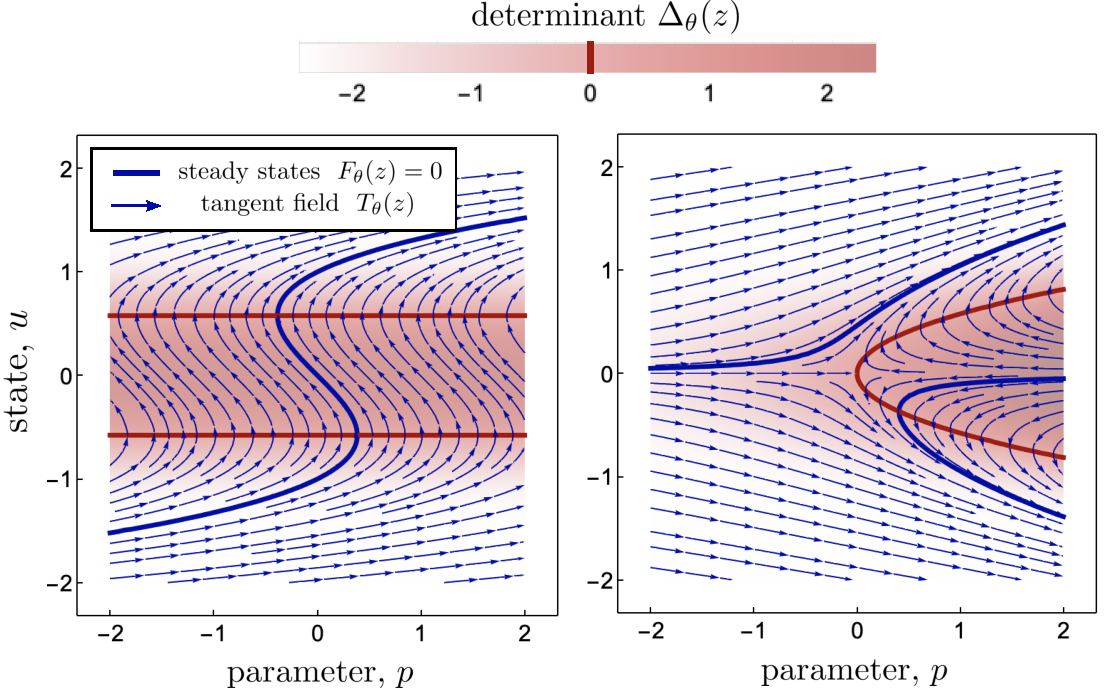
\includegraphics[width=13cm]{determinant-field}
\caption{Left/Right : Determinant $\Det$ and tangent field $\tangent(z)$ for the saddle-node/pitchfork models for some set values of $\theta$ revealing that $\Det=0$ defines bifurcations}
\label{fig:determinant-field}
\end{figure}
Figure \ref{fig:determinant-field} shows how the bifurcation curve defined by $\rates(z)=0$ picks out one of many level sets or traces in tangent field $\tangent(z)$ for the saddle and pitchfork. The tangent field $\tangent(z)$ can always be analytically evaluated by taking the determinant in \eqref{eq:tangent-field}. We will proceed with calculations on $\tangent(z)$ in the whole space $z$ and pick out a single trace by solving $\rates(z)=0$ later. For our two models
\begin{align}
    \underset{\mathrm{saddle-node\,\,model}}{
    \tangent(z)=\hat{u}-(\,3\theta_2 u^2+\theta_1\,)\,\hat{p}}
    \qquad\qquad
    \underset{\mathrm{pitchfork\,\,model}}{
    \tangent(z)=u\hat{u}-(\,3\theta_2 u^2+p\,)\,\hat{p}}
    \label{eq:tangent-field-examples}
\end{align}
Figure \ref{fig:determinant-field} reveals that $\Det=0$ is also a level set and that the intersection with level set $\rates(z)=0$ defines the bifurcations at specific parameter $\theta$. In this particular setting we can see that the tangent field $\tangent(z)$ only folds when $\Det=0$. Plotting the value of the determinant along $\rates(z)=0$ from Figure \ref{fig:determinant-field} would give rise to Figures \ref{fig:minimal-models}. The directional derivative of the determinant $\Det$ along the tangent field $\tangent(z)$ is defined as
\begin{align}
    \frac{d}{ds}\Det := \hat{\tangent}(z) \cdot \frac{\partial}{\partial z}\Det 
\end{align}
where $\hat{\tangent}(z)$ is the unit tangent field. 


\section{Bifurcation Measure}
\label{appendix:measure}


\section{Simplification of two-state model}

Consider the general two-state model:
\begin{equation}
    \dfrac{dv_i}{dt} = \dfrac{a_i + b_i (K_i v_j)^2}{1 + (K_i v_j)^2} - \mu_i v_i
\end{equation}

Without loss of generality, we can rescale $v_i = U_i u_i$. Then,
\begin{equation}
    \dfrac{U_idu_i}{dt} = \dfrac{a_i + b_i (K_i U_j u_j)^2}{1 + (K_i U_j u_j)^2} - \mu_i U_i u_i
\end{equation}

Dividing through by $U_i$, we obtain
\begin{equation}
    \dfrac{du_i}{dt} = \dfrac{\frac{a_i}{U_i} + \frac{b_i}{U_i} (K_i U_j u_j)^2}{1 + (K_i U_j u_j)^2} - \mu_i u_i
\end{equation}

By choosing $U_i = b_i$, the model reduces to:
\begin{equation}
    \dfrac{du_1}{dt} = \dfrac{\hat{a}_1 + (p u_2)^2}{1 + (p u_2)^2} - \mu_1 u_1, \quad
    \dfrac{du_2}{dt} = \dfrac{\hat{a}_2 + (k u_1)^2}{1 + (k u_1)^2} - \mu_2 u_2
\end{equation}
where $p = \frac{K_1}{\sqrt{b_1}}$ and $k = \frac{K_2}{\sqrt{b_2}}$.



\bibliography{refs}
\bibliographystyle{ieeetr}
\end{document}
